\chapter{Termo de Abertura do projeto}

\section{EAP}
\begin{figure}[!htb]
    \center{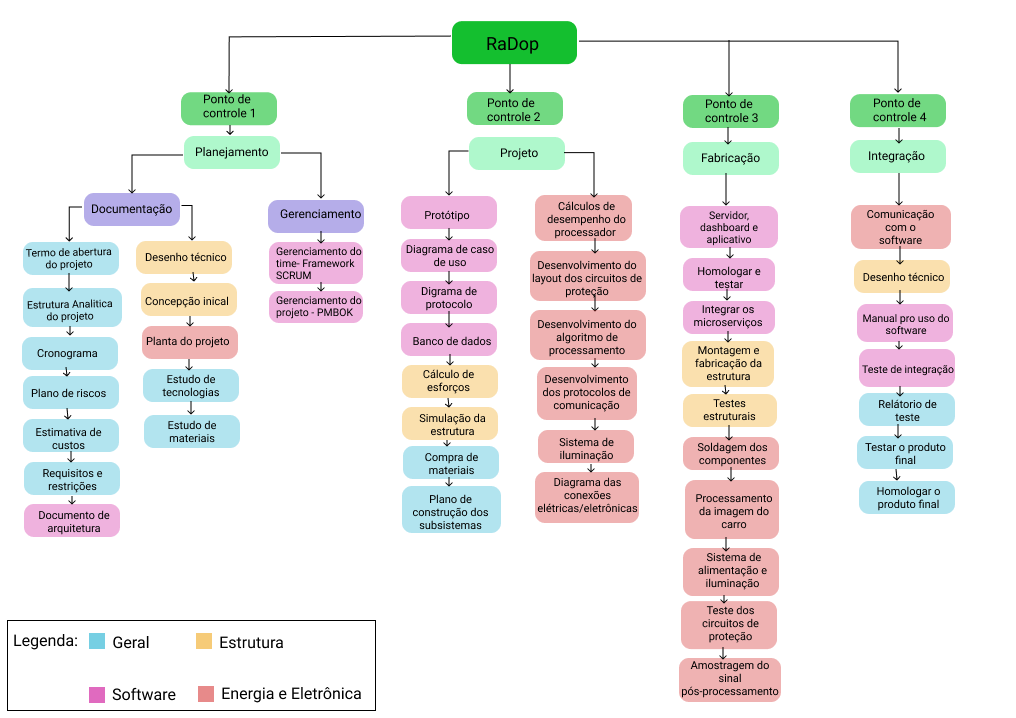
\includegraphics[width=\textwidth]{eap}}
    \caption{\label{fig:eap} EAP do projeto}
\end{figure}
\section{Lista É/Não é}
\subsection{É}
\subsection{Não é}
\section{Requisitos}
\subsection{Eletrônica}
\subsection{Energia}
\subsection{Estrutura}
\subsection{Software}

Os requisistos de software são:

\begin{itemize}
    \item Interface do Dashboard;
    \item Interface do Aplicativo;
    \item Manual de uso dos softwares (Microsserviços, Aplicativo e Dashboard);
    \item Funcionar com conexão a redes (Internet);
    \item Ser capaz de lidar e recuperar de falhas e erros (conexão, processamento e etc.);
    \item Softwares devem ser manuteníveis e evolutíveis;
    \item Softwares devem ser testáveis e testados;
    \item Software deve mostrar dados e informações do Radar;
    \item Software deve ser capaz de tomar decisões para alertar socorristas a respeito de prováveis acidentes automobilísticos;
    \item Software deve ser capaz de tomar decisões para alertar usuários de possíveis situações de risco;
    \item Software deve ser capaz de mostrar informações gerenciais com os dados do Radar;
\end{itemize}

As restrições de software são:

\begin{itemize}
    \item O software necessita estar sempre conectado à internet para comunicação e, consequentemente, para o correto funcionamento;
    \item O aplicativo de manutenção irá auxiliar apenas com o essencial;
    \item O aplicativo só funcionará em aparelhos Android;
    \item A linguagem de cada microsserviço (assim como framework/tecnologia) será definida dada necessidade (performance, armazemanento e etc) dos mesmos;
\end{itemize}

\section{\emph{Stakeholders}}
\section{Recurso humanos}

 De modo a ter uma melhor organização, a equipe foi dividida em subgrupos, onde cada subgrupo tem um gerente técnico, além disso a equipe também conta com um gerente de qualidade e um coordenador geral. Na Figura \ref{fig:organograma} mostra o organograma da equipe e o nome de cada integrante por função.
 
\begin{figure}[h]
\centering
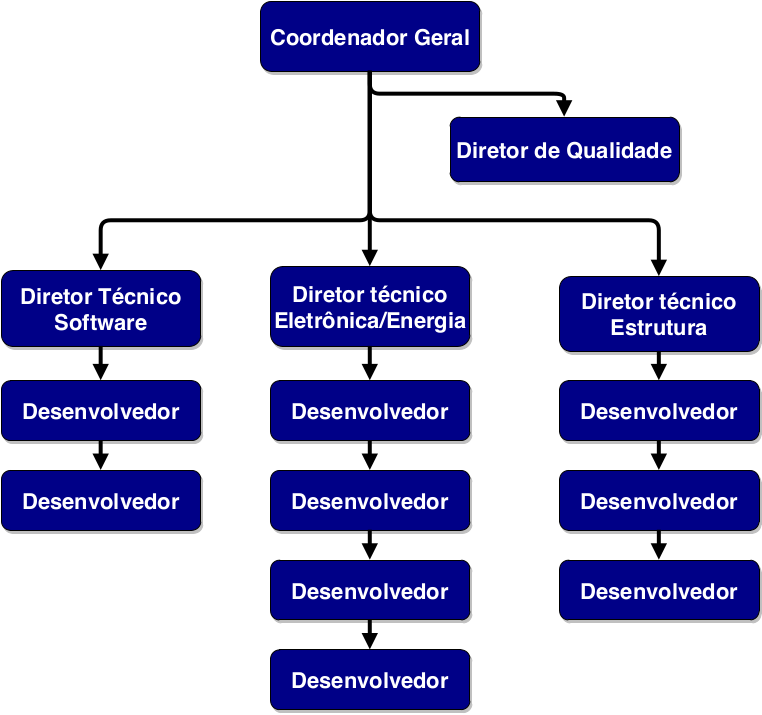
\includegraphics[scale = 0.5]{organograma.pdf}
\caption{.}\label{fig:organograma}
\end{figure} 

A seguir estão os nomes de cada integrante separado por área:

\begin{itemize}
\item Eletrônica e Energia

-Brenda Bianca Neves Dias\\
-Danyelle Bemfica da Rocha\\
-\textbf{Elpidio Cândido de Araújo Bisneto -> Coordenador geral}\\
-Filipe de Souza Freitas\\
-\textbf{Kewin Kuster -> Diretor técnico}\\
-Rodrigo Sousa Santos

\item Estrutura

-\textbf{Daniele Dias Sousa -> Diretora de qualidade}\\
-Fernanda Resende Muro Martinez\\
-Luiz Felipe Martins Cruz\\
-Pedro Henrique Nazareno Halabi\\
-\textbf{Rafael Mascarenhas dos Santos -> Diretor técnico}

\item Software

-Diego Barbosa da Mota França\\
-\textbf{João Pedro Sconetto -> Diretor técnico}\\
-Mariana Mendes 


\end{itemize}

\subsection{Ferramentas de gerenciamento}

Foram selecionadas algumas ferramentas de gerenciamento, afim de organizar o trabalho da equipe.

\emph{\textbf{Discord:}} É um aplicativo de comunicação onde a equipe pode se comunicar de forma rápida com mensagens, além disso permite o envio de vídeos, imagens e documentos. Outra vantagem da ferramenta é a possibilidade de fazer áudio-conferência com mais de 10 pessoas.

\emph{\textbf{Google drive:}} Ferramenta em nuvem para armazenamento e compartilhamento de arquivos.

\emph{\textbf{GitHub e Texmaker:}} \emph{Texmaker} é uma ferramenta para edição de texto em \emph{Latex} e o \emph{GitHub} é um ferramenta de desenvolvimento.

\emph{\textbf{Trello:}} O Trello é bastante conhecido por ser uma ferramenta de gerenciamento de projetos. 

\section{Cronograma de atividades}
\section{Milestones Identificados}
\section{Estimativa de custos}

\subsection{Engenharia de Software}

Aqui está listado todos os gastos que serão necessários para a equipe de software, assim como todas as aquisições que serão feitas durante o projeto:

\begin{table}[h]
    \resizebox{\textwidth}{!}{\begin{tabular}{@{}|c|c|c|c|c|c|c|@{}}
    \toprule
    \textbf{Nome do produto} & \textbf{Descrição}                      & \textbf{Marca} & \textbf{Preço unitário} & \textbf{Quantidade} & \textbf{Fornecedor} & \textbf{Orçamento} \\ \midrule
    Servidor                 & Máquina para execução dos serviços      & ---            & US\$ 10,00 por mês      & 5 meses             & Digital Ocean       & US\$ 50,00         \\ \midrule
    Raspberry Pi 3 B         & Placa de IoT para execução de softwares & Raspberry      & R\$ 279,90              & 1 unidade           & FilipeFlop          & R\$ 279,90         \\ \bottomrule
    \end{tabular}}
\end{table}

OBS: Essa planilha poderá ser atualizado dependendo de necessidades que surgirem durante a execução do projeto.

\section{Viabilidades financeira}
\section{Levantamento de riscos}
